% !TeX root = ./eLife_draft.tex

%%%%%%%%%%%%%%%%%%%%%%%%%%%%%%%%%%%%%%%%%%%%%%%%%%%%%%%%%%%%
%%% ELIFE ARTICLE TEMPLATE
%%%%%%%%%%%%%%%%%%%%%%%%%%%%%%%%%%%%%%%%%%%%%%%%%%%%%%%%%%%%
%%% PREAMBLE 
\documentclass[9pt,lineno]{elife}
% Use the onehalfspacing option for 1.5 line spacing
% Use the doublespacing option for 2.0 line spacing
% Please note that these options may affect formatting.
% Additionally, the use of the \newcommand function should be limited.

\usepackage{lipsum} % Required to insert dummy text
\usepackage[version=4]{mhchem}
\usepackage{siunitx}
\DeclareSIUnit\Molar{M}

%%%%%%%%%%%%%%%%%%%%%%%%%%%%%%%%%%%%%%%%%%%%%%%%%%%%%%%%%%%%
%%% ARTICLE SETUP
%%%%%%%%%%%%%%%%%%%%%%%%%%%%%%%%%%%%%%%%%%%%%%%%%%%%%%%%%%%%

\title{Fundamental limits on the rate of bacterial cell division}
\author[1, *]{Nathan M. Belliveau}
\author[2, 3, *]{Griffin Chure}
\author[4]{Christina L. Hueschen}
\author[5]{Hernan G. Garcia}
\author[6]{Jan\'{e} Kondev}
\author[1, 7]{Julie Theriot}
\author[1, 8, $\dagger$]{Rob Phillips}
\affil[1]{Department of Biology, University of Washington, Seattle, WA, USA}
\affil[2]{Division of Biology and Biological Engineering, California Institute of Technology, Pasadena, CA, USA}
\affil[3]{Department of Applied Physics, California Institute of Technology, Pasadena, CA, USA}
\affil[4]{Department of Chemical Engineering, Stanford University, Stanford, CA, USA}
\affil[5]{Department of Molecular Cell Biology and Department of Physics, University of California Berkeley, Berkeley, CA, USA}
\affil[6]{Department of Physics, Brandeis University, Waltham, MA, USA}
\affil[7]{Allen Institute for Cell Science, Seattle, WA, USA}
\affil[8]{Department of Physics, California Institute of Technology, Pasadena, CA, USA}
\affil[$\dagger$]{Address correspondence to phillips@pboc.caltech.edu}
\affil[*]{Contributed equally}

\contrib[*]{These authors contributed equally to this work}

%%%%%%%%%%%%%%%%%%%%%%%%%%%%%%%%%%%%%%%%%%%%%%%%%%%%%%%%%%%%
%%% ARTICLE START
%%%%%%%%%%%%%%%%%%%%%%%%%%%%%%%%%%%%%%%%%%%%%%%%%%%%%%%%%%%%

\begin{document}

\maketitle

\begin{abstract}

\end{abstract}

% !TeX root = ./eLife_draft.tex

\section{Introduction}
The observed range of bacterial growth rates is enormously diverse. In natural
environments, some microbial organisms may double only once per year
\citep{mikucki2009} while in comfortable laboratory conditions, growth can be
rapid with several divisions per hour \citep{schaechter1958}. This six
order-of-magnitude difference in time scales of growth encompasses different
microbial species and lifestyles, yet even for a single species such as
\textit{Escherichia coli}, the growth rate can be modulated over a
large scale by tuning the type and amount of nutrients in the growth medium
\citep{liu2005a}. This remarkable plasticity in growth rate illustrates the
intimate relationship between environmental conditions and the rates at which
cells convert nutrients into new cellular material -- a relationship that has
remained a major topic of inquiry in bacterial physiology for over a century
\citep{jun2018}.

A key discovery in bacterial physiology of the past 70 years was the
identification of bacterial "growth laws" \citep{schaechter1958}; empirical
relationships that relate the bacterial growth rate to the protein and RNA
composition of the intracellular milieu in a number of different species.
Over the past decade, a flurry of work \citep{molenaar2009, scott2010,
klumpp2014, basan2015, dai2016, erickson2017} has examined these growth laws
at a quantitative level, developing a series of phenomenological models from
which the growth laws naturally emerge. In parallel, a "molecular revolution"
in biology has yielded an increasingly refined molecular census of the cell,
particularly for bacteria such as the microbial workhorse \textit{E. coli}
\citep{schmidt2016, davidi2016a}. In light of the now expansive trove of
quantitative biological data, we can revisit several of the evergreen
questions about bacterial growth and physiology that were originally raised
by microbiologists in the middle of the 20th century. Specifically, what
biological processes are the primary determinants for how quickly bacterial
cells can grow and reproduce? Why do cells modulate the absolute numbers and
relative ratios of their molecular constituents as a function of changes in
growth rate or nutrient availability?

In this work, we begin by considering these two questions from two distinct
angles. First, as a result of an array of high-quality proteome-wide
measurements of \textit{E. coli} under diverse growth conditions, we have
generated a census that allows us to explore how the number of key molecular
players change as a function of growth rate. Here, we have assembled a singular
data set of protein copy numbers using measurements collected over the past
decade via mass spectrometry \citep{schmidt2016, peebo2015, valgepea2013} or
ribosomal profiling \citep{li2014} of the composition of the \textit{E. coli}
proteome across a gamut of growth rates. Due to notable changes in cell size and
cellular composition as a function of growth rate \citep{bremer2008,
taheriaraghi2015}, as well as differences in normalization and standardization
schemes used in each experimental work, substantial care was taken to ensure
consistency on a per cellular basis (see the Appendix for a detailed analysis
and additional discussion). To our knowledge, this compiled and curated dataset
represents the most comprehensive view to date of the \textit{E. coli} proteome,
covering $\approx$ 4000 proteins and 36 unique growth rates, with the observed
abundance of any given protein being directly comparable between data sets and
across growth rates. This allows us to interrogate  the \textit{E. coli}
specific physiology underlying the observed abundances while  minimizing the
effects of experimental noise, as  $\approx$ 75\% of the  proteins are observed
in at least two separate datasets.

Second, by compiling molecular turnover rate measurements for many of the
fundamental processes associated with bacterial growth, we make quantitative
estimates of a handful of key cellular processes (schematized in
\FIG{categories}) to determine whether our current understanding of the
kinetics of these processes are sufficient to explain the magnitude of the
observed protein copy numbers across conditions (see \BOX{estimate_rules}
describing the philosophy behind this approach). The census, combined with
these estimates, provide a window into the question of whether the rates of
central processes such as energy generation or DNA synthesis vary
systematically as a function of cell growth rate by altering protein copy
number.

Throughout our estimates, we consider an archetypal growth rate of $\approx$
0.5 hr$^{-1}$ corresponding to a doubling time of $\approx$ 5000 seconds, as
the data sets examined here heavily sample this growth regime. While we
formulate point estimates for the protein abundances at this division time,
we also consider how these values will vary at other growth rates due to
changes in cell size, surface area, and chromosome copy number
\citep{taheriaraghi2015, harris2018}. For the majority of the processes
considered, we find that the protein copy numbers appear tuned for the task
of cell doubling across a continuum of growth rates. Thus, our understanding
of the kinetics of various biological processes is sufficient to
quantitatively explain the observed abundances of these proteins.

% From these estimates, it emerges that translation, particularly the synthesis of
% ribosomal proteins, is a plausible candidate that limits the rate of cellular
% growth in \textit{E. coli}.

From these estimates, it emerges that translation,  particularly the synthesis of ribosomal proteins is a
plausible candidate that limits the rate of cellular growth in \textit{E. coli}.
We reach this conclusion by considering that ribosome synthesis is 1) a rate
limiting step for the \textit{fastest} bacterial division, and  2) the main
determinant of bacterial growth rate across  nutrient conditions associated with
moderate to fast growth rates. In addition, a strict dependence between the
maximal growth rate and ribosomal mass fraction coincides with the regime where
the growth laws appear most valid \citep{amir2017, scott2010}. This enables us
to suggest that the long-observed correlation between growth rate and cell size
\citep{schaechter1958, si2017} can be simply attributed to the increased
absolute number of ribosomes per cell under conditions supporting extremely
rapid growth. To better understand how the observed alterations in absolute
protein abundances, and in particular, changes in ribosome copy number,
influence growth rate across different nutrient conditions we consider a minimal
model of cellular growth. Our conclusions from these analyses provide important
insight into how \textit{E. coli} regulates growth across conditions of
differing nutrient availability and identifies fundamental constraints in
bacterial growth more broadly.






\begin{figure}
    \centering{
    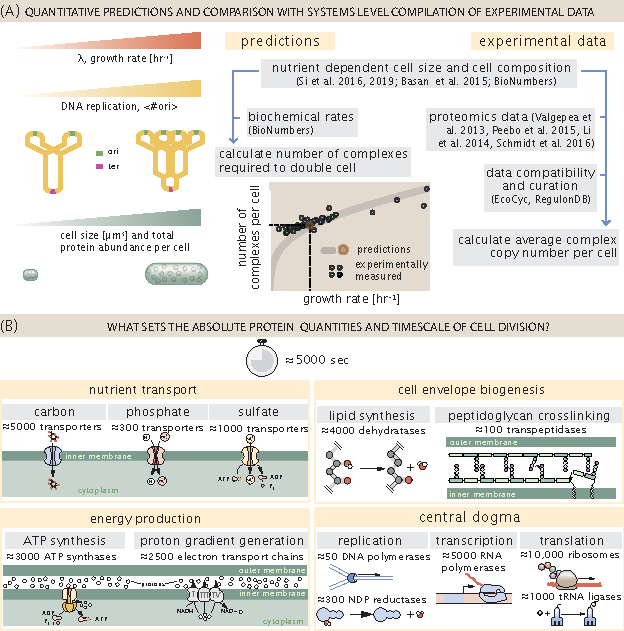
\includegraphics{main_figs/fig1_schematic_categories_grouped.pdf}
    \caption{\textbf{Transport and synthesis processes necessary for cell division.}
            We consider an array of processes necessary for a cell to double its
            molecular components, broadly grouped into four classes. These
            categories are (A) nutrient transport across the cell membrane, (B) cell envelope
            biogenesis, (C) energy production (namely, ATP synthesis), and (D) processes associated with the central dogma.
            Numbers shown are the approximate number of complexes of each type
            observed at a growth rate of 0.5 hr$^{-1}$, or a cell doubling time
            of $\approx$ 5000 s.}
    \label{fig:categories}
    }
\end{figure}




% \begin{table}[bt]
% \caption{\label{tab:example}Automobile Land Speed Records (GR 5-10).}
% % Use "S" column identifier to align on decimal point 
% \begin{tabular}{S l l l r}
% \toprule
% {Speed (mph)} & Driver          & Car                        & Engine    & Date     \\
% \midrule
% 407.447     & Craig Breedlove & Spirit of America          & GE J47    & 8/5/63   \\
% 413.199     & Tom Green       & Wingfoot Express           & WE J46    & 10/2/64  \\
% 434.22      & Art Arfons      & Green Monster              & GE J79    & 10/5/64  \\
% 468.719     & Craig Breedlove & Spirit of America          & GE J79    & 10/13/64 \\
% 526.277     & Craig Breedlove & Spirit of America          & GE J79    & 10/15/65 \\
% 536.712     & Art Arfons      & Green Monster              & GE J79    & 10/27/65 \\
% 555.127     & Craig Breedlove & Spirit of America, Sonic 1 & GE J79    & 11/2/65  \\
% 576.553     & Art Arfons      & Green Monster              & GE J79    & 11/7/65  \\
% 600.601     & Craig Breedlove & Spirit of America, Sonic 1 & GE J79    & 11/15/65 \\
% 622.407     & Gary Gabelich   & Blue Flame                 & Rocket    & 10/23/70 \\
% 633.468     & Richard Noble   & Thrust 2                   & RR RG 146 & 10/4/83  \\
% 763.035     & Andy Green      & Thrust SSC                 & RR Spey   & 10/15/97\\
% \bottomrule
% \end{tabular}

% \tabledata{This is a description of a data source.}

% \end{table}







% For a half-width figure or table with text wrapping around it, use 

% \begin{verbatim}
% \begin{wrapfigure}{l}{.46\textwidth}
%   \includegraphics[width=\hsize]{...}
%   \caption{...}\label{...}
% \end{wrapfigure}
% \end{verbatim}
% %
% as in \FIG{halfwidth}. For tables:

% If you use the following prefixes for your \verb|\label|:
% %
% \begin{description}
% \item[Figures] \texttt{fig:}, e.g.~\verb|\label{fig:view}|
% \item[Figure Supplements] \texttt{figsupp:}, e.g.~\verb|\label{figsupp:sf1}|\\
% (we'll assume \texttt{figsupp:sf1} is a figure supplement of \texttt{fig:view} in our example)
% \item[Figure source data] \texttt{figdata:}, e.g.~\verb|\label{figdata:first}|
% \item[Videos] \texttt{video:}, e.g.~\verb|\label{video:mv1}|
% \item[Video supplements] \texttt{videosupp:}, e.g.~\verb|\label{videosupp:sv1}|
% \item[Tables] \texttt{tab:}, e.g.~\verb|\label{tab:example}|
% \item[Equations] \texttt{eq:}, e.g.~\verb|\label{eq:CLT}|
% \item[Boxes] \texttt{box:}, e.g.~\verb|\label{box:simple}|
% \end{description}
% %
% you can then use the convenience commands \verb|\FIG{view}|, \verb|\FIGSUPP[view]{sf1}|, \verb|\TABLE{example}|, \verb|\EQ{CLT}|, \verb|\BOX{simple}|, \verb|\FIGDATA[view]{first}|, \verb|\VIDEO{mv1}| and \verb|{\VIDEOSUPP}[view]{sv1}| \emph{without} the label prefixes, to generate cross-references \FIG{view}, \FIGSUPP[view]{sf1},  \TABLE{example}, \EQ{CLT}, \BOX{simple}, \FIGDATA[view]{first}, \VIDEO{mv1} and \VIDEOSUPP[view]{sv1}. Alternatively, use \verb|\autoref| with the full label, e.g.~\autoref{first:app} (although this may not work correctly for figures and tables in the appendices or boxes nor supplements at present).

% Really wide figures or tables, that take up the entire page, including the gutter space: use \verb|\begin{fullwidth}...\end{fullwidth}| as in \FIG{fullwidth}. And sometimes you may want to use feature boxes like \BOX{simple}.

% \begin{wrapfigure}{l}{.46\textwidth}
% 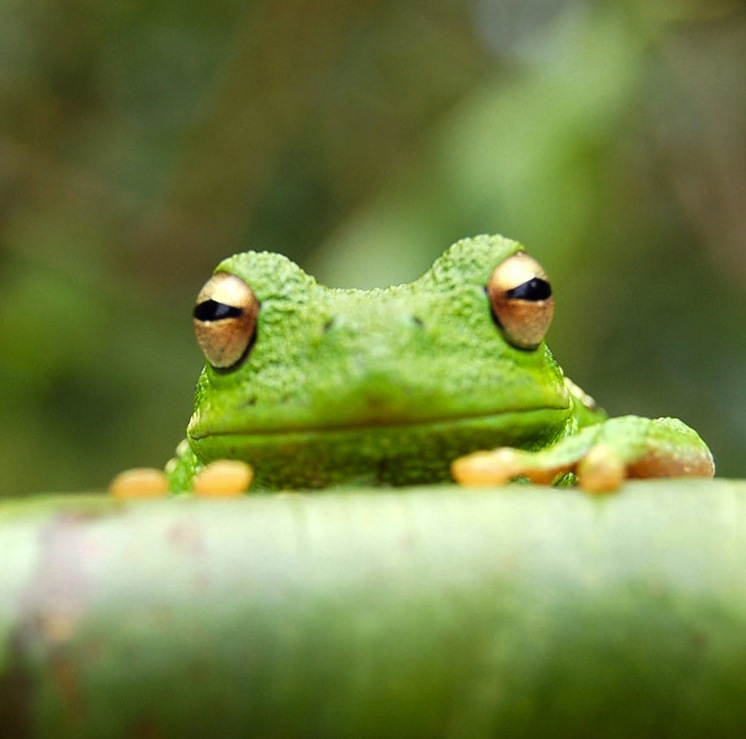
\includegraphics[width=\hsize]{frog}
% \caption{A half-columnwidth image using wrapfigure, to be used sparingly. Note that using a wrapfigure before a sectional heading, near other floats or page boundaries is not recommended, as it may cause interesting layout issues. Use the optional argument to wrapfigure to control how many lines of text should be set half-width alongside it.}
% \label{fig:halfwidth}
% \end{wrapfigure}


% \begin{figure}
% \begin{fullwidth}
% 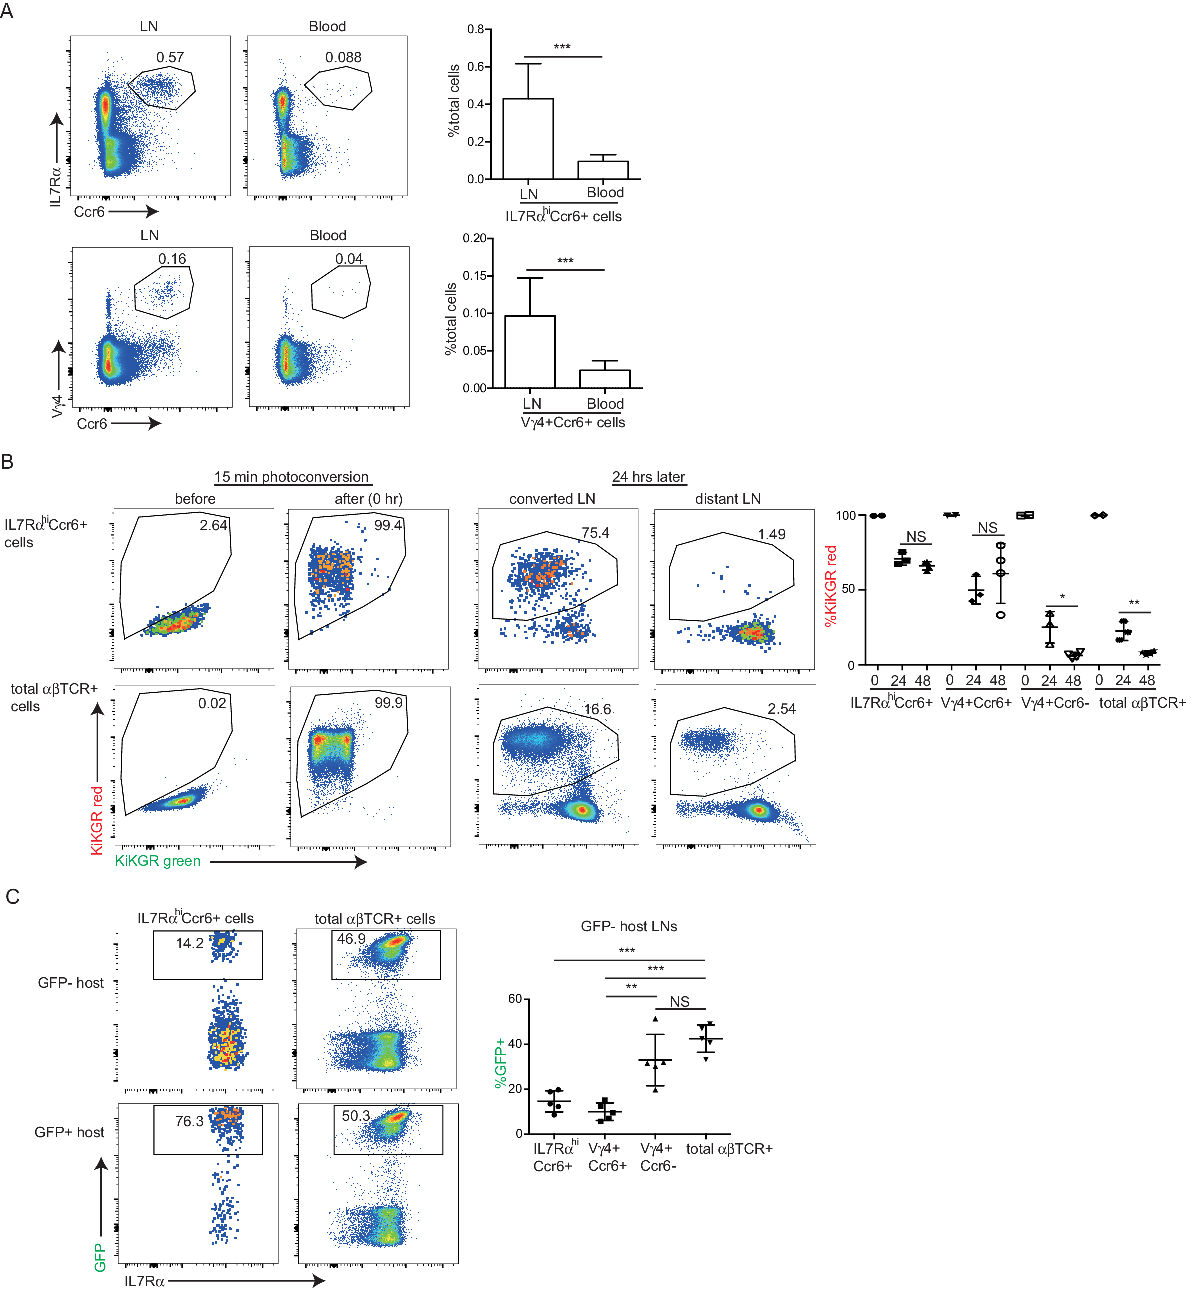
\includegraphics[width=0.95\linewidth]{elife-18156-fig2}
% \caption{A very wide figure that takes up the entire page, including the gutter space.}
% \label{fig:fullwidth}
% \figsupp{There is no limit on the number of Figure Supplements for any one primary figure. Each figure supplement should be clearly labelled, Figure 1--Figure Supplement 1, Figure 1--Figure Supplement 2, Figure 2--Figure Supplement 1 and so on, and have a short title (and optional legend). Figure Supplements should be referred to in the legend of the associated primary figure, and should also be listed at the end of the article text file.}{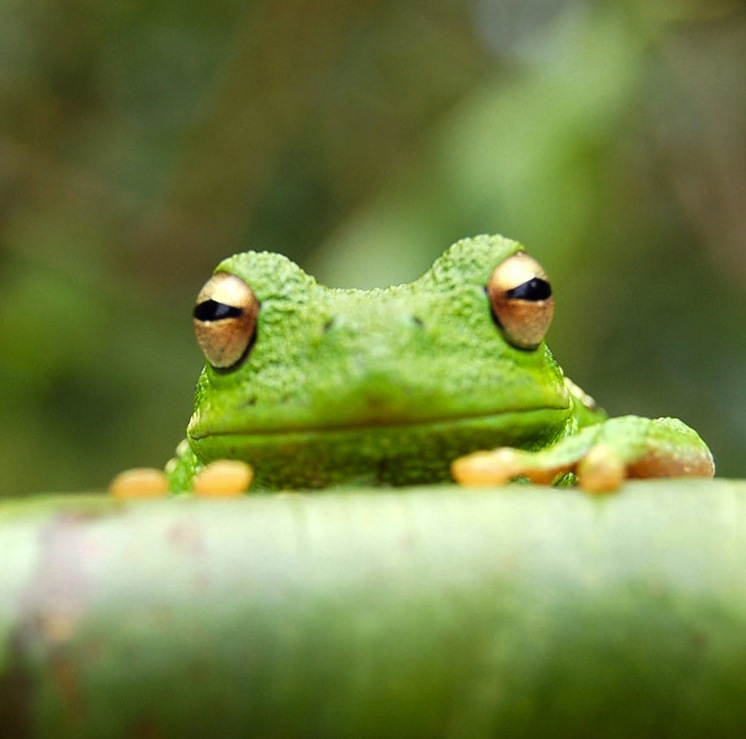
\includegraphics[width=5cm]{frog}}
% \end{fullwidth}
% \end{figure}


% \figsupp[Shorter caption for main text.]{This is a supplementary figure's full caption, which will be used at the end of the manuscript.}{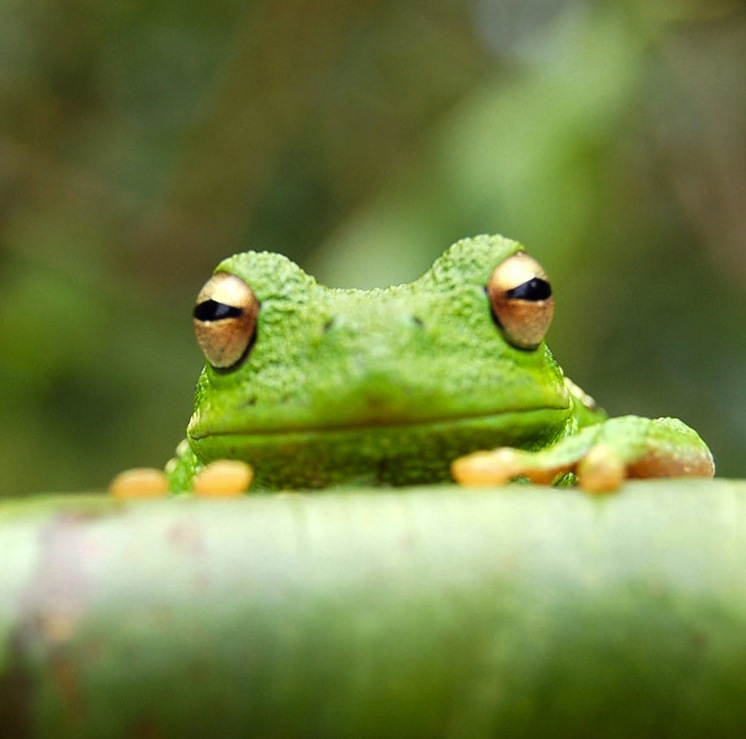
\includegraphics[width=6cm]{frog}}\label{figsupp:sf1}
% \figsupp{This is another supplementary figure.}{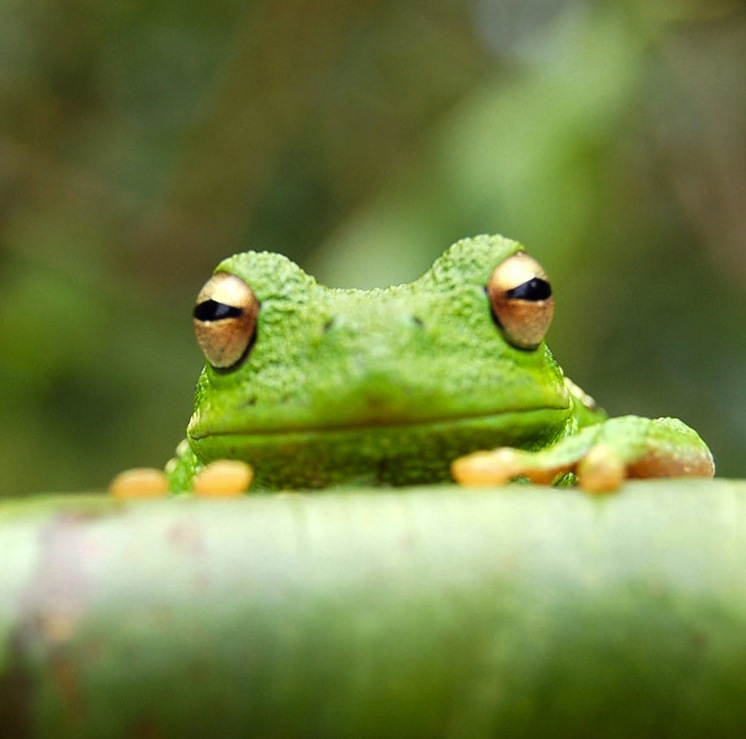
\includegraphics[width=6cm]{frog}}
% \videosupp{This is a description of a video supplement.}\label{videosupp:sv1}
% \figdata{This is a description of a data source.}\label{figdata:first}
% \figdata{This is another description of a data source.}\label{figdata:second}






% \section{Acknowledgments}

% Additional information can be given in the template, such as to not include funder information in the acknowledgments section.

% \nocite{*} % This command displays all refs in the bib file. PLEASE DELETE IT BEFORE YOU SUBMIT YOUR MANUSCRIPT!
\bibliography{library.bib}

%%%%%%%%%%%%%%%%%%%%%%%%%%%%%%%%%%%%%%%%%%%%%%%%%%%%%%%%%%%%
\end{document}